\documentclass[12pt]{article}
 
\usepackage[margin=1in]{geometry} 
\usepackage{amsmath,amsthm,amssymb}
\usepackage{float}
\usepackage{tikz}
\usetikzlibrary{arrows,shapes,trees} % loads some tikz extensions
 
\begin{document}
 
\title{Homework 2}
\author{Josh Klontz
CSE 802}
 
\maketitle

\begin{enumerate}
\item \textbf{Solve the following problems from Chapter 2 of the textbook: 8, 10, 14 Parts (a), (b), and (c), 24}
  \subitem \textbf{8. Let the conditional densities for a two-category one-dimensional problem be given by the Cauchy distribution described in Problem 7.}
  \begin{enumerate}
  \item \textbf{By explicit integration, check that the distributions are indeed normalized.}
    \begin{figure}[H]
    \begin{equation}
      p(x|w_i) = \frac{1}{\pi b} \cdot \frac{1}{1 + (\frac{x-a_i}{b})^2}
    \end{equation}
    \caption{Probability density function of a Cauchy distribution.}
    \end{figure}
    The probability density is considered to be normalized if it integrates to 1:
    \begin{equation}
    \begin{split}
      \int_{-\infty}^{\infty} p(x|w_i) dx& = \int_{-\infty}^{\infty} \frac{1}{\pi b} \cdot \frac{1}{1 + (\frac{x-a_i}{b})^2} dx \\
      & = \frac{1}{\pi b} \int_{-\infty}^{\infty} \frac{1}{1 + (\frac{x-a_i}{b})^2} dx
    \end{split}
    \end{equation}
    Apply U-substituion:
    \begin{equation}
    \begin{split}
      u& = \frac{x-a_i}{b} \\
      & = \frac{x}{b} \cdot \frac{a_i}{b} \\
    \frac{du}{dx}& = \frac{1}{b} \\
    dx& = b\ du
    \end{split}
    \end{equation}
    To obtain:
    \begin{equation}
    \begin{split}
      \int_{-\infty}^{\infty} p(x|w_i) dx& = \frac{1}{\pi} \int_{-\infty}^{\infty} \frac{1}{1 + u^2} du \\
      & = \frac{1}{\pi} \cdot tan^{-1}(u) |_{-\infty}^{\infty} \\
      & = \frac{1}{\pi} (\frac{\pi}{2} - \frac{-\pi}{2}) \\
      & = \frac{1}{\pi} \pi \\
      & \boxed{= 1}
    \end{split}
    \end{equation}
  \item \textbf{Assuming that $P(w_1) = P(w_2)$, show that $P(w_1|x) = P(w_2|x)$ if $x = (a_1 + a_2)/2$.}
    \begin{equation}
    \begin{split}
      P(w_1|x)& \iff P(w_2|x) \\
      \frac{p(x|w_1)P(w_1)}{p(x)}& \iff \frac{p(x|w_2)P(w_2)}{p(x)} \\
      p(x|w_1)P(w_1)& \iff p(x|w_2)P(w_2) \\
      p(x|w_1)& \iff p(x|w_2) \\
      \frac{1}{\pi b} \cdot \frac{1}{1 + (\frac{x-a_1}{b})^2}& \iff \frac{1}{\pi b} \cdot \frac{1}{1 + (\frac{x-a_2}{b})^2} \\
      \frac{1}{1 + (\frac{x-a_1}{b})^2}& \iff \frac{1}{1 + (\frac{x-a_2}{b})^2} \\
      1 + (\frac{x-a_1}{b})^2& \iff 1 + (\frac{x-a_2}{b})^2 \\
      (\frac{x-a_1}{b})^2& \iff (\frac{x-a_2}{b})^2 \\
      \frac{x^2-2xa_1+a_1^2}{b^2}& \iff \frac{x^2-2xa_2+a_2^2}{b^2} \\
      x^2-2xa_1+a_1^2& \iff x^2-2xa_2+a_2^2 \\
      -2xa_1+a_1^2& \iff -2xa_2+a_2^2 \\
      -2(\frac{a_1+a_2}{2})a_1 + a_1^2& \iff -2(\frac{a_1+a_2}{2})a_2 + a_2^2 \\
      -(a_1+a_2)a_1 + a_1^2& \iff -(a_1+a_2)a_2 + a_2^2 \\
      (a_1+a_2)a_2 + a_1^2& \iff (a_1+a_2)a_1 + a_2^2 \\
      a_1^2+ a_1a_2 + a_2^2 & = a_1^2+ a_1a_2 + a_2^2 \\
      & \qed
    \end{split}
    \end{equation}
  \item \textbf{Plot $P(w_1|x)$ for the case $a_1=3, a_2=5, b=1$.}
    \begin{equation}
    \begin{split}
      P(w_1|x)& = \frac{p(x|w_1)P(w_1)}{p(x)} \\
      & = \frac{\frac{1}{\pi b} \cdot \frac{1}{1 + (\frac{x-a_1}{b})^2} \cdot 0.5}{\frac{1}{\pi b} \cdot \frac{1}{1 + (\frac{x-a_1}{b})^2} \cdot 0.5 + \frac{1}{\pi b} \cdot \frac{1}{1 + (\frac{x-a_2}{b})^2} \cdot 0.5} \\
      & = \frac{\frac{1}{1 + (\frac{x-a_1}{b})^2}}{\frac{1}{1 + (\frac{x-a_1}{b})^2} + \frac{1}{1 + (\frac{x-a_2}{b})^2}} \\
      & = \frac{1 + (\frac{x-a_2}{b})^2}{1 + (\frac{x-a_1}{b})^2 + 1 + (\frac{x-a_2}{b})^2} \\
      & = \frac{1 + (x-a_2)^2}{2b^2 + (x-a_1)^2 + (x-a_2)^2} \\
      & = \frac{b^2 + (x-a_2)^2}{2b^2 + (x-a_1)^2 + (x-a_2)^2} \\
      & = \frac{1 + (x-5)^2}{2 + (x-3)^2 + (x-5)^2} \\
      & = \frac{x^2 - 10x + 26}{2x^2-16x+36}
    \end{split}
    \end{equation}
    \begin{figure}[H]
      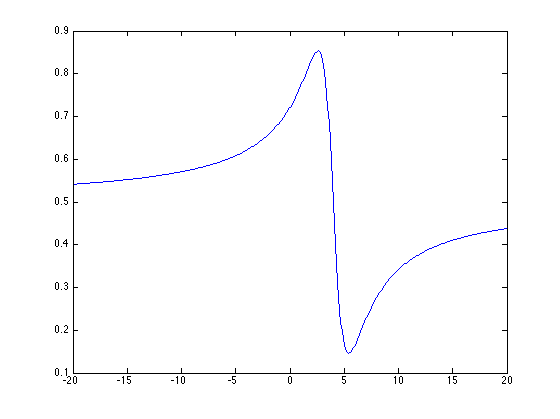
\includegraphics[width=\textwidth]{8c}
    \end{figure}
  \item \textbf{How do $P(w_1|x)$ and $P(w_2|x)$ behave as $x \rightarrow -\infty$ and $x \rightarrow +\infty$? Explain.} \\
    $P(w_1|x)$ and $P(w_2|x)$ approach $\frac{1}{2}$. This is because they have the same variance and their difference in means is decreasingly important as $x \rightarrow \pm \infty$.
  \end{enumerate}
  \subitem{\textbf{10. Consider the following decision rule for a two-category one-dimensional problem: Decide $w_1$ if $x>\theta$; otherwise decide $w_2$.}}
  \begin{enumerate}
  \item \textbf{Show that the probability of error for this rule is given by}
    \begin{equation}
      P(error) = P(w_1)\int_{-\infty}^\theta p(x|w_1)dx + P(w_2) \int_\theta^\infty p(x|w_2)dx
    \end{equation}
    \begin{equation}
    \begin{split}
      P(error)& = \int_{-\infty}^\infty 1-p(w_{decision}|x)dx \\
      & = \int_{-\infty}^\theta 1-p(w_2|x)dx + \int_\theta^\infty 1-p(w_1|x)dx \\
      & = \int_{-\infty}^\theta p(w_1|x)dx + \int_\theta^\infty p(w_2|x)dx \\
      & = \int_{-\infty}^\theta \frac{p(x|w_1)P(w_1)}{p(x)}dx + \int_\theta^\infty \frac{p(x|w_2)P(w_2)}{p(x)}dx \\
      & = P(w_1)\int_{-\infty}^\theta \frac{p(x|w_1)}{1}dx + P(w_2)\int_\theta^\infty \frac{p(x|w_2)}{1}dx \\
      & \boxed{= P(w_1)\int_{-\infty}^\theta p(x|w_1)dx + P(w_2) \int_\theta^\infty p(x|w_2)dx}
    \end{split}
    \end{equation}
  \item \textbf{By differentiating, show that a necessary condition to minimize $P(error)$ is that $\theta$ satisfies}
    \begin{equation}
      p(\theta|w_1)P(w_1)=p(\theta|w_2)P(w_2)
    \end{equation}
    \begin{equation}
    \begin{split}
      \left(P(w_1)\int_{-\infty}^\theta p(x|w_1)dx + P(w_2) \int_\theta^\infty p(x|w_2)dx\right) d\theta& = 0 \\
      P(w_1)\int_{-\infty}^\theta p(x|w_1)dxd\theta + P(w_2) \int_\theta^\infty p(x|w_2)dxd\theta& = 0 \\
      P(w_1)(-p(\theta|w_1)) + P(w_2)(p(\theta|w_2))& = 0 \\
      p(\theta|w_1)P(w_1)& =p(\theta|w_2)P(w_2) \\
      & \qed
    \end{split}
    \end{equation}
  \item \textbf{Does this equation satisfy $\theta$ uniquely?} \\
    No, there may exist multiple values of theta corresponding to multiple optimal decision boundaries based on the underlying probability density functions.
  \item \textbf{Given an example where a value of $\theta$ satisfying the equation actually \emph{maximizes} the probability of error.} \\
    Consider the trivial case where $P(w_1)=P(w_2)$ and $p(x|w_1)=p(x|w_2)$. In this case, all values of $\theta$ maximize the probability of error.
  \end{enumerate}
  \subitem \textbf{14. Consider the classification problem with rejection option.}
  \begin{enumerate}
  \item \textbf{Use the results of problem 13 to show that the following discriminant functions are optimal for such problems:}
    \begin{equation}
      g_i(x) = \left\{ \begin{array}{ll}p(x|w_i)P(w_i) & i = 1, ..., c \\ \frac{\lambda_s-\lambda_r}{\lambda_s}\sum_{j=1}^c p(x|w_j)P(w_j) & i = c+1 \end{array} \right.
    \end{equation}
The optimal desciminant functions maximize the negative risk:
    \begin{equation}
    \begin{split}
      g_i(x)& = \left\{ \begin{array}{ll}-\lambda_s (1-P(w_i|x)) & i = 1, ..., c \\ -\lambda_r & i = c+1 \end{array} \right. \\
      & = \left\{ \begin{array}{ll}-\lambda_s + \lambda_s P(w_i|x)) & i = 1, ..., c \\ -\lambda_r & i = c+1 \end{array} \right. \\
      & = \left\{ \begin{array}{ll}\lambda_s P(w_i|x)) & i = 1, ..., c \\ \lambda_s -\lambda_r & i = c+1 \end{array} \right. \\
      & = \left\{ \begin{array}{ll}P(w_i|x)) & i = 1, ..., c \\ \frac{\lambda_s -\lambda_r}{\lambda_s} & i = c+1 \end{array} \right. \\
      & = \left\{ \begin{array}{ll}\frac{p(x|w_i)P(w_i)}{p(x)} & i = 1, ..., c \\ \frac{\lambda_s -\lambda_r}{\lambda_s} & i = c+1 \end{array} \right. \\
      & = \left\{ \begin{array}{ll}p(x|w_i)P(w_i) & i = 1, ..., c \\ \frac{\lambda_s -\lambda_r}{\lambda_s}p(x) & i = c+1 \end{array} \right. \\
      & \boxed{= \left\{ \begin{array}{ll}p(x|w_i)P(w_i) & i = 1, ..., c \\ \frac{\lambda_s-\lambda_r}{\lambda_s}\sum_{j=1}^c p(x|w_j)P(w_j) & i = c+1 \end{array} \right.}
    \end{split}
    \end{equation}
  \item \textbf{Plot these disciminant functions and the decision regions for the two-category one-dimensional case having}
    \begin{equation}
    \begin{split}
      g_1& = \frac{1}{2\sqrt{2\pi}}e^{-\frac{1}{2}(x-1)^2} \\
      g_2& = \frac{1}{2\sqrt{2\pi}}e^{-\frac{1}{2}(x+1)^2} \\
      g_3& = \frac{g_1 + g_2}{2}
    \end{split}
    \end{equation}
    \begin{figure}[H]
      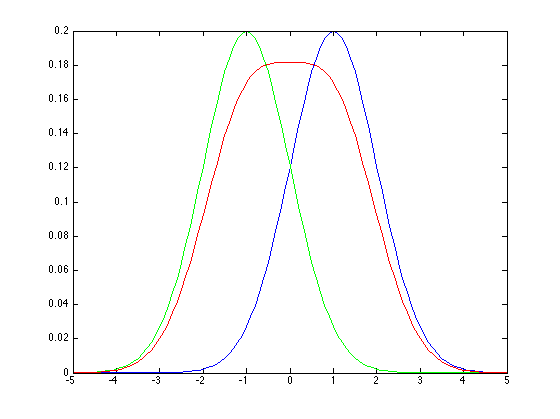
\includegraphics[width=\textwidth]{14b}
      \caption{$g_1 = blue$, $g_2 = green$, $g_3 = red$. Decision boundaries at $g_1 = g_3$ and $g_2 = g_3$.}
    \end{figure}
  \item \textbf{Describe qualitatively what happens as $\lambda_r/\lambda_s$ is increased from 0 to 1.} \\
  When $\lambda_r/\lambda_s = 0$ there is no cost associated with the rejection option and it should be taken every time. As $\lambda_r/\lambda_s$ increases, the size of the $g_3$ distribution shrinks with respect to $g_1$ and $g_2$, and the decision region where the rejection option should be taken becomes increasingly narrow. When $\lambda_r/\lambda_s = 1$ there is no instance where it is optimal to take the rejection option.
  \end{enumerate}
  \subitem \textbf{24. Consider the multivariate normal density with mean $\mu$, $\sigma_{ij}=0$ and $sigma_{ii}=\sigma_i^2$}
  \begin{enumerate}
  \item \textbf{Show that the evidence is}
    \begin{equation}
      p(\mathbf{x}) = \frac{1}{\prod_{i=1}^d \sqrt{2\pi}\sigma_i} \exp\left[-\frac{1}{2}\sum_{i=1}^d\left(\frac{x_i-\mu_i}{\sigma_i}\right)^2\right]
    \end{equation}
    \begin{equation}
    \begin{split}
      p(\mathbf{x})& = \frac{1}{(2\pi)^{d/2}|\boldsymbol{\Sigma}|^{1/2}} \exp\left[-\frac{1}{2}(\mathbf{x}-\boldsymbol{\mu})^t\boldsymbol{\Sigma}^{-1}(\mathbf{x}-\boldsymbol{\mu})\right] \\
      & = \frac{1}{(2\pi)^{d/2}(\prod_{i=1}^d\sigma_i^2)^{1/2}} \exp\left[-\frac{1}{2}(\mathbf{x}-\boldsymbol{\mu})^t\boldsymbol{\Sigma}^{-1}(\mathbf{x}-\boldsymbol{\mu})\right] \\
      & = \frac{1}{(2\pi)^{d/2}\prod_{i=1}^d\sigma_i} \exp\left[-\frac{1}{2}(\mathbf{x}-\boldsymbol{\mu})^t\boldsymbol{\Sigma}^{-1}(\mathbf{x}-\boldsymbol{\mu})\right] \\
      & = \frac{1}{\prod_{i=1}^d \sqrt{2\pi}\sigma_i} \exp\left[-\frac{1}{2}(\mathbf{x}-\boldsymbol{\mu})^t\boldsymbol{\Sigma}^{-1}(\mathbf{x}-\boldsymbol{\mu})\right] \\
      & = \frac{1}{\prod_{i=1}^d \sqrt{2\pi}\sigma_i} \exp\left[-\frac{1}{2}\sum_{i=1}^d\left((x_i-\mu_i) \cdot \frac{1}{\sigma_i^2} \cdot (x_i-\mu_i)\right)^2\right] \\
      & = \frac{1}{\prod_{i=1}^d \sqrt{2\pi}\sigma_i} \exp\left[-\frac{1}{2}\sum_{i=1}^d\left(\frac{x_i-\mu_i}{\sigma_i}\right)^2\right]
    \end{split}
    \end{equation}
  \item \textbf{Plot and describe the contours of constant density.}
    \begin{figure}[H]
      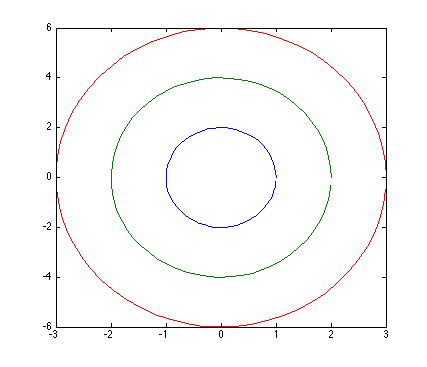
\includegraphics[width=\textwidth]{24b}
      \caption{The contours of constant density are ellipses centered at mean $\boldsymbol{\mu}$. The ellipses are oriented parallel to the underlying vector space but the magnitude of each axis is independent.}
    \end{figure}
  \item \textbf{Write an expression for the Mahalanobis distance from $\mathbf{x}$ to $\boldsymbol{\mu}$.}
    \begin{equation}
    \begin{split}
      r& = \sqrt{(\mathbf{x}-\boldsymbol{\mu})^t\boldsymbol{\Sigma}^{-1}(\mathbf{x}-\boldsymbol{\mu})} \\
      & = \sqrt{\sum_{i=1}^d\left((x_i-\mu_i) \cdot \frac{1}{\sigma_i^2} \cdot (x_i-\mu_i)\right)^2} \\
      & \boxed{= \sqrt{\sum_{i=1}^d\left(\frac{x_i-\mu_i}{\sigma_i}\right)^2}}
    \end{split}
    \end{equation}
  \end{enumerate}
\item \textbf{Consider a two-category classification problem with two-dimensional
feature vector $X = (x1, x2)$. The two categories are $w_1$ and $w_2$.}
  \begin{enumerate}
  \item \textbf{Find the maximum likelihood and Bayes decision rules. Express
them as functions of $x_1$ and $x_2$.}
    \begin{figure}[H]
    \begin{equation}
    \begin{split}
      LR& = \frac{p(X|w_1)}{p(X|w_2)} \\
      & = \frac{\frac{1}{(2\pi)^{d/2}|\boldsymbol{\Sigma_1}|^{1/2}} \exp\left[-\frac{1}{2}(\mathbf{x}-\boldsymbol{\mu_1})^t\boldsymbol{\Sigma_1}^{-1}(\mathbf{x}-\boldsymbol{\mu_1})\right]}{\frac{1}{(2\pi)^{d/2}|\boldsymbol{\Sigma_2}|^{1/2}} \exp\left[-\frac{1}{2}(\mathbf{x}-\boldsymbol{\mu_2})^t\boldsymbol{\Sigma_2}^{-1}(\mathbf{x}-\boldsymbol{\mu_2})\right]} \\
      & = \frac{|\boldsymbol{\Sigma_2}|^{1/2} \exp\left[\frac{1}{2}(\mathbf{x}-\boldsymbol{\mu_2})^t\boldsymbol{\Sigma_2}^{-1}(\mathbf{x}-\boldsymbol{\mu_2})\right]}{|\boldsymbol{\Sigma_1}|^{1/2} \exp\left[\frac{1}{2}(\mathbf{x}-\boldsymbol{\mu_1})^t\boldsymbol{\Sigma_1}^{-1}(\mathbf{x}-\boldsymbol{\mu_1})\right]} \\
      & = \frac{|[\begin{array}{ll}1&1\\1&2\end{array}]|^{1/2} \exp\left[\frac{1}{2}([\begin{array}{l}x_1\\x_2\end{array}]-[\begin{array}{c}1\\-2\end{array}])^t[\begin{array}{ll}1&1\\1&2\end{array}]^{-1}([\begin{array}{l}x_1\\x_2\end{array}]-[\begin{array}{c}1\\-2\end{array}])\right]}{|[\begin{array}{ll}2&1\\1&1\end{array}]|^{1/2} \exp\left[\frac{1}{2}([\begin{array}{l}x_1\\x_2\end{array}]-[\begin{array}{c}1\\2\end{array}])^t[\begin{array}{ll}2&1\\1&1\end{array}]^{-1}([\begin{array}{l}x_1\\x_2\end{array}]-[\begin{array}{c}1\\2\end{array}])\right]} \\
      & = \frac{\exp\left[\frac{1}{2}[\begin{array}{l}x_1-1\\x_2+2\end{array}]^t[\begin{array}{cc}2&-1\\-1&1\end{array}][\begin{array}{l}x_1-1\\x_2+2\end{array}]\right]}{\exp\left[\frac{1}{2}[\begin{array}{l}x_1-1\\x_2-2\end{array}]^t[\begin{array}{cc}1&-1\\-1&2\end{array}]^{-1}[\begin{array}{l}x_1-1\\x_2-2\end{array}]\right]} \\
      & = \frac{[\begin{array}{l}x_1-1\\x_2+2\end{array}]^t[\begin{array}{cc}2&-1\\-1&1\end{array}][\begin{array}{l}x_1-1\\x_2+2\end{array}]}{[\begin{array}{l}x_1-1\\x_2-2\end{array}]^t[\begin{array}{cc}1&-1\\-1&2\end{array}][\begin{array}{l}x_1-1\\x_2-2\end{array}]} \\
      & = \frac{[\begin{array}{l}2x_1-x_2-4\\-x_1+x_2+3\end{array}]^t[\begin{array}{l}x_1-1\\x_2+2\end{array}]}{[\begin{array}{l}x_1-x_2+1\\-x_1+2x_2-3\end{array}]^t[\begin{array}{l}x_1-1\\x_2-2\end{array}]} \\
      & = \frac{(2x_1-x_2-4)(x_1-1)+(-x_1+x_2+3)(x_2+2)}{(x_1-x_2+1)(x_1-1)+(-x_1+2x_2-3)(x_2-2)} \\
      & = \frac{2x_1^2-x_1x_2-6x_1+x_2+4-x_1x_2+x_2^2+5x_2-2x_1+6}{x_1^2-x_1x_2+x_2-1-x_1x_2+2x_2^2-7x_2+2x_1+6} \\
      & = \frac{2x_1^2+x_2^2-2x_1x_2-8x_1+6x_2+10}{x_1^2+2x_2^2-2x_1x_2+2x_1-6x_2+5} \\
      g & = (x_1^2+2x_2^2-2x_1x_2+2x_1-6x_2+5)-(2x_1^2+x_2^2-2x_1x_2-8x_1+6x_2+10) \\
      g & = \boxed{-x_1^2+x_2^2+10x_1-12x_2-5}
    \end{split}
    \end{equation}
    \caption{Maximum likelihood decision rule: $w_2$ if $g > 0$, $w_1$ otherwise.}
    \end{figure}
    \begin{figure}[H]
    \begin{equation}
    \begin{split}
      LR& = \frac{p(X|w_1)P(w_1)}{p(X|w_2)P(w_2)} \\
      & ... \\
      g & = P(w_2)(x_1^2+2x_2^2-2x_1x_2+2x_1-6x_2+5)-P(w_1)(2x_1^2+x_2^2-2x_1x_2-8x_1+6x_2+10) \\
      g & = 0.7(x_1^2+2x_2^2-2x_1x_2+2x_1-6x_2+5)-0.3(2x_1^2+x_2^2-2x_1x_2-8x_1+6x_2+10) \\
      g & = \boxed{0.1x_1^2+1.1x_2^2-0.8x_1x_2+3.8x_1-6x_2+0.5}
    \end{split}
    \end{equation}
    \caption{Bayes decision rule: $w_2$ if $g > 0$, $w_1$ otherwise.}
    \end{figure}
  \item \textbf{Generate 500 patterns from each of the two class-conditional densities using the mvnrnd function in MATLAB, and plot them in the two-dimensional feature space, using the plot function. Also plot the two decision boundaries obtained in 2(a) on the same figure.}
    \begin{figure}[H]
      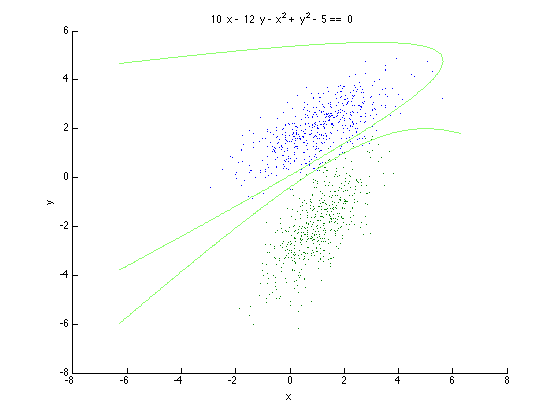
\includegraphics[width=\textwidth]{2b}
    \end{figure}
  \item \textbf{Generate 50 additional test patterns from each class and determine the empirical error values corresponding to the two decision boundaries.}
    \begin{table}[H]
    \centering
    \begin{tabular}{lcc}
      & Maximum Likelihood & Bayes \\
      $w_1$ & 0\% & 2\% \\
      $w_2$ & 0\% & 0\% \\
    \end{tabular}
    \caption{Empirical error rates.}
    \end{table}
  \item \textbf{Calculate the Bhattacharya error bound and compare the empirical error values obtained in 2(c) with the error bound.}
    \begin{equation}
    \begin{split}
      k(1/2)& = 1/8(\mu_2-\mu_1)^t\left[\frac{\Sigma_1+\Sigma_2}{2}\right]^{-1}(\mu_2-\mu_1)+\frac{1}{2} \ln\frac{|\frac{\Sigma_1+\Sigma_2}{2}|}{\sqrt{|\Sigma_1||\Sigma_2|}} \\
      & = 1/8([\begin{array}{c}1\\-2\end{array}]-[\begin{array}{c}1\\2\end{array}])^t\left[\frac{[\begin{array}{cc}2&1\\1&1\end{array}]+[\begin{array}{cc}1&1\\1&2\end{array}]}{2}\right]^{-1}([\begin{array}{c}1\\-2\end{array}]-[\begin{array}{c}1\\2\end{array}])+\frac{1}{2} \ln\frac{|\frac{[\begin{array}{cc}2&1\\1&1\end{array}]+[\begin{array}{cc}1&1\\1&2\end{array}]}{2}|}{\sqrt{|[\begin{array}{cc}2&1\\1&1\end{array}]||[\begin{array}{cc}1&1\\1&2\end{array}]|}} \\
      & = 1/8[\begin{array}{c}0\\-4\end{array}]^t\left[\frac{[\begin{array}{cc}3&2\\2&3\end{array}]}{2}\right]^{-1}[\begin{array}{c}0\\-4\end{array}]+\frac{1}{2} \ln|\frac{[\begin{array}{cc}3&2\\2&3\end{array}]}{2}| \\
      & = 1/8[\begin{array}{c}0\\-4\end{array}]^t[\begin{array}{cc}1.5&1\\1&1.5\end{array}]^{-1}[\begin{array}{c}0\\-4\end{array}]+\frac{1}{2} \ln|[\begin{array}{cc}1.5&1\\1&1.5\end{array}]| \\
      & = 1/8[\begin{array}{c}0\\-4\end{array}]^t[\begin{array}{cc}1.2&-.8\\-.8&1.2\end{array}][\begin{array}{c}0\\-4\end{array}]+\frac{1}{2} \ln(1.25) \\
      & = 1/8[\begin{array}{c}3.2\\-4.8\end{array}]^t[\begin{array}{c}0\\-4\end{array}]+.112 \\
      & = 1/8(19.2)+.112 \\
      & = 2.4 + .112 \\
      & = 2.512 \\
      P(error)& = P(w_1)P(w_2)e^{-k(1/2)} \\
      & = 0.3 \cdot 0.7 \cdot e^{-2.512} \\
      & \boxed{= 0.017}
    \end{split}
    \end{equation}
  \end{enumerate}
  Bhattacharya bound is tight with respect to the empirical error rates.
\item \textbf{Construct a table defining all possible decision rules for this problem. For example, one of the possible decision rule is: If a test pattern x = 1, take action α1; if x = 2, take action α2; if x = 3,
take action α3. Compute the posterior probabilities and find the optimal Bayes decision rule without considering the loss function. Now compute the conditional risk for each rule. How does the optimal decision rule change when the loss function is taken into account?}
  \begin{equation}
  \begin{split}
    p(x_1)& = 0.2*0.4 + 0.3*0.3 + 0.6*0.3 \\
    & = 0.35 \\
    p(x_2)& = 0.1*0.4 + 0.5*0.3 + 0.2*0.3 \\
    & = 0.25 \\
    p(x_3)& = 0.7*0.4 + 0.2*0.3 + 0.2*0.3 \\
    & = 0.4 \\
  \end{split}
  \end{equation}
  \begin{table}[H]
  \centering
  \begin{tabular}{ccccc}
    & $w_1$ & $w_2$ & $w_3$ \\
    x=1 & 0.2*0.4/0.35 & 0.3*0.3/0.35 & 0.6*0.3/0.35 \\
    x=2 & 0.1*0.4/0.25 & 0.5*0.3/0.25 & 0.2*0.3/0.25 & \\
    x=3 & 0.7*0.4/0.4 & 0.2*0.3/0.4 & 0.2*0.3/0.4 &
  \end{tabular}
  \\
  \begin{tabular}{ccccc}
    & $w_1$ & $w_2$ & $w_3$ \\
    x=1 & 0.229 & 0.257 & \textbf{0.514} \\
    x=2 & 0.16 & \textbf{0.6} & 0.24 & \\
    x=3 & \textbf{0.7} & 0.15 & 0.15 &
  \end{tabular}
  \caption{Posterior probabilities with optimal Bayes decision rule shown in bold.}
  \end{table}
  \begin{table}[H]
  \centering
  \begin{tabular}{ccccc}
    & $a_1$ & $a_2$ & $a_3$ & $a_4$ \\
    x=1 & 0.257*2+0.514*5 & 0.229*1+0.514*1 & 0.229*3+0.257*2 & 0.229*2+0.257*3+0.514*1\\
    x=2 & 0.6*2+0.24*5 & 0.16*1+0.24*1 & 0.16*2+0.6*3 & 0.16*2+0.6*3+0.24*1 \\
    x=3 & 0.15*2+0.15*5 & 0.7*1+0.15*1 & 0.7*3+0.15*2 & 0.7*2+0.15*3+0.15*1
  \end{tabular}
  \\
  \begin{tabular}{ccccc}
    & $a_1$ & $a_2$ & $a_3$ & $a_4$ \\
    x=1 & 3.084 & \textbf{0.743} & 1.201 & 1.743\\
    x=2 & 2.4 & \textbf{0.4} & 2.12 & 2.36 \\
    x=3 & 1.05 & \textbf{0.85} & 2.4 & 2
  \end{tabular}
  \caption{Conditional risk with optimal decision rule shown in bold. $w_2$ becomes the optimal decision rule for all values of $x$ because of its low risk.}
  \end{table}
\end{enumerate}
\end{document}
